\documentclass[ai,article,submit,oneauthor]{Definitions/mdpi}

\usepackage{amsfonts}
\usepackage{bm}
\usepackage{threeparttable}
\usepackage{listings}
\usepackage{xcolor}

\definecolor{positivegain}{RGB}{0, 90, 180} 
\definecolor{negativegain}{RGB}{190, 30, 45} 
\newcommand{\posgain}[1]{\textcolor{positivegain}{#1}} 
\newcommand{\neggain}[1]{\textcolor{negativegain}{#1}} 
\newcommand{\sigposgain}[1]{\textcolor{positivegain}{\textbf{#1}}} 
\newcommand{\signeggain}[1]{\textcolor{negativegain}{\textbf{#1}}}
\newcommand{\sigposci}[1]{\textcolor{positivegain}{#1}}
\newcommand{\signegci}[1]{\textcolor{negativegain}{#1}}

\setlength{\headheight}{24pt}

\graphicspath{{figures/}}

\newcommand{\selfrefine}{Self-Refine}
\newcommand{\selfdebug}{Self-Debug}
\newcommand{\pp}{percentage points}
\newcommand{\todo}[1]{\textcolor{red}{[TODO: #1]}}
\newcommand{\researchquestion}[2]{%
    \par\medskip
    \noindent\textbf{#1.} \textit{#2}\par
    \smallskip
}

% Model names used throughout the paper
\newcommand{\gptthreefive}{GPT-3.5}
\newcommand{\gptfouromini}{GPT-4o mini}
\newcommand{\gptfouro}{GPT-4o}
\newcommand{\gptfivesixsol}{GPT-5.6 Sol}
\newcommand{\qwentwofive}{Qwen2.5}
\newcommand{\deepseekvtwo}{DeepSeek-V2}
\newcommand{\qwenthreecoder}{Qwen3-Coder}
\newcommand{\modelentry}[2]{%
    \textbf{#1}\newline
    {\scriptsize #2}%
}
\newcommand{\rqanswer}[2]{%
    \begin{center}
    \fbox{\parbox{0.92\columnwidth}{%
        \textbf{Answer to #1.} #2}}
    \end{center}    
}

\lstdefinestyle{prompt}{
basicstyle=\ttfamily\scriptsize,
frame=single,
breaklines=true,
breakindent=0pt,
breakautoindent=false,
columns=fullflexible,
keepspaces=true,
showstringspaces=false,
aboveskip=6pt,
belowskip=6pt,
xleftmargin=3pt,
xrightmargin=3pt,
framexleftmargin=3pt,
framexrightmargin=3pt,
captionpos=b
}

\firstpage{1}
\makeatletter
\setcounter{page}{\@firstpage}
\makeatother
\pubvolume{1}
\issuenum{1}
\articlenumber{0}
\pubyear{2026}
\copyrightyear{2026}
\datereceived{}
\daterevised{}
\dateaccepted{}
\datepublished{}

\Title{Evaluating Self-Refinement Protocols for Code Generation: Explicit Critique, Revision Planning, and Decision-Conditioned Refinement}
\Author{Jindae Kim $^{1,*}$}
\AuthorNames{Jindae Kim}
\address{%
$^{1}$ \quad Department of Computer Science and Engineering, Seoul National University of Science and Technology, Seoul 01811, Republic of Korea; jindae.kim@seoultech.ac.kr}
\corres{Correspondence: jindae.kim@seoultech.ac.kr}

\abstract{
Abstract.
}

\keyword{large language models; code generation; self-refinement; self-refinement protocol; self-critique}

\begin{document}

\input{sections/01_intro}
\section{Background}

Self-Refinement improves an Initial Candidate through one or more subsequent model calls.
Self-Refine established a general pattern in which the same large language model (LLM) generates an output, produces natural-language feedback, and revises the output without additional training \cite{madaan2023selfrefine}.
In code generation, Self-Debugging prompts the model to explain and revise its own code and, when unit tests are available, also uses execution results as feedback \cite{chen2024selfdebug}.
We use Self-Refinement in a narrower sense: the same model reviews and revises its Self-Generated Initial Candidate using only the task specification and self-generated intermediate artifacts, while tests are reserved for post-hoc evaluation and no Execution Feedback is provided to the model.

\subsection{Challenges and Risks of Code Self-Refinement}

An additional refinement call does not necessarily produce a better program.
Olausson et al. compare self-repair with independent resampling at an equivalent program-sampling budget and find modest or absent gains in several settings; stronger-model and human feedback improve repair, indicating that feedback quality is a key bottleneck \cite{olausson2024selfrepair}.
For locally run 1-3B models, Feedback Over Form finds that execution feedback and early stopping drive improvements, while its constrained topology search provides no clear gain over a simple refinement loop \cite{mcandrews2026feedback}.
Its exploratory text-only pipeline experiments show no improvement, but the study treats them as secondary, less systematic evidence \cite{mcandrews2026feedback}.
Although both studies examine repair with execution feedback, they motivate evaluating whether the benefits of additional refinement calls justify their cost.

Refinement can also damage an initially correct program.
CoCoS explicitly reports incorrect-to-correct and correct-to-incorrect transitions and trains small models to maintain correct outputs while improving incorrect ones \cite{cho-etal-2025-self}.
This transition-based view is close to our analysis, but CoCoS trains a correction-preserving model rather than comparing inference-time protocols over the same Initial Candidate.
CodeChat-Eval provides complementary evidence by finding statistically significant declines in Functional Correctness across ten-turn sessions of functionality-preserving follow-up instructions \cite{guo2026codechateval}.
Its revisions follow curated developer-preferred instructions rather than self-generated critique, but the observed regressions demonstrate that more editing is not inherently beneficial.

A refinement system must therefore decide not only how to revise a candidate, but also whether the candidate should be revised.
Jin and Chen show that, when judging requirement conformance without executing tests, LLMs frequently reject correct implementations and justify these decisions with invented requirements, excessive edge-case concerns, or unsupported claims \cite{jin2026reliable}.
Such overcorrection may trigger unnecessary refinement, although a false review verdict does not by itself establish a Correct-to-Incorrect Regression in the revised code.
Revisit Self-Debugging finds that post-execution repair can be misled by bias in self-generated tests, showing that apparently informative test feedback may still provide an unreliable basis for repair \cite{chen-etal-2025-revisit}.
These findings motivate paired analysis of Repair, Correct-to-Incorrect Regression, and exact preservation instead of relying only on final pass rate.

\subsection{Methods for Improving Code Self-Refinement}

One family of methods improves refinement through explicit critique or reflection.
RCO trains a critic with a critique-utility reward derived from the improvement of an actor's revised response, avoiding direct critique-preference assessment \cite{yu-etal-2025-training}.
SCOPE adapts a prover model into a structured critic that produces subgoals, gap analysis, and a robustness checklist to guide code correction \cite{zhang2026scope}.
Broader reflection systems include Reflexion, which stores verbal reflections on task feedback in episodic memory \cite{shinn2023reflexion}, and INDICT, which coordinates safety- and helpfulness-oriented critics equipped with external knowledge and tools \cite{le2024indict}.
These methods support the idea that an explicit critique or reflection artifact can guide subsequent decisions, but they use trained critics, external signals and tools, or integrated agent loops rather than isolating the effect of adding Critique and Planning to a fixed model.

Other methods learn correction behavior or structure pre-execution review.
SCoRe trains self-correction with two-stage, multi-turn online reinforcement learning under the model's own distribution of self-generated correction traces \cite{kumar2025score}, whereas CoCoS adapts multi-turn reinforcement learning to small models through accumulated and progressive rewards \cite{cho-etal-2025-self}.
ReflexiCoder internalizes initial generation, bug- and optimization-aware reflection, and self-correction in the model weights, avoiding an execution engine at inference time \cite{jiang-etal-2026-reflexicoder}.
ReVISE uses a preference-learning curriculum to train self-verification and reasoning correction sequentially \cite{pmlr-v267-lee25ab}, while RubricRefine generates task- and tool-registry-specific rubrics to check semantic contracts and repair tool-use code before execution \cite{levine2026rubricrefine}.
These approaches show that correction and verification can be learned or structured, but their integrated procedures do not expose the incremental correctness and token effects of separate inference-time Refinement Stages.
Code Reffix uses oracle reflections and a dual-task protocol to decouple the evaluation of reflection generation from reflection-guided repair \cite{di-etal-2026-code}, and CodeReviewQA decomposes review comprehension into change-type recognition, change localization, and solution identification \cite{lin-etal-2025-codereviewqa}.
The COAST study evaluates bug localization, identification, repair, and recognition through DEBUGEVAL and uses communicative agents to synthesize debugging data for training \cite{yang-etal-2025-coast}.
These decompositions provide indirect support for Stage Composition, while focusing on capability evaluation or training rather than Shared-Initial protocol comparison.

A second family improves refinement with Execution Feedback.
Self-Edit supplies example-test execution results to a fault-aware editor \cite{zhang-etal-2023-self}, while CYCLE trains models to refine faulty generations from available feedback, including test-suite execution results \cite{ding2024cycle}.
LeDex trains on explanation-and-refinement trajectories filtered through execution verification \cite{jiang2024ledex}, and OpenCodeInterpreter supports iterative code generation and refinement using execution and human feedback \cite{zheng-etal-2024-opencodeinterpreter}.
More detailed signals are used by LDB, which tracks and verifies runtime states at the basic-block level \cite{zhong-etal-2024-debug}, and by TraceCoder, which uses runtime traces for diagnosis, repair, and rollback \cite{huang2026tracecoder}.
CodeT instead selects among generated solutions using generated tests and dual execution agreement \cite{chen2023codet}, whereas LEVER reranks generated programs with an execution-aware verifier \cite{pmlr-v202-ni23b}; neither method revises a single Initial Candidate.
These methods demonstrate the value of behavioral evidence for debugging, but their results cannot determine how well a model refines code without execution feedback or external verification.

Multi-agent and repository-level systems place refinement within broader workflows: AgentCoder separates programming, test design, and test execution \cite{huang2023agentcoder}; MapCoder separates example recall, planning, code generation, and debugging \cite{islam-etal-2024-mapcoder}; RepairAgent autonomously selects tools for program repair \cite{bouzenia2025repairagent}; and Agentless reduces repository repair to localization, repair, and patch validation \cite{xia2024agentless}.
Their stage and resource tradeoffs therefore include execution or repository interaction that is absent from our fixed-candidate setting.
Adjacent work also includes InterCode, which formalizes interactive coding as reinforcement-learning environments where execution feedback is observed after code actions \cite{yang2023intercode}, and RefineCoder, which iteratively retrains code models on data refined from self-generated code and external critiques \cite{zhou2025refinecoder}.
SemCoder trains models to reason about statement-level execution effects and program behavior \cite{ding2024semcoder}, while CRITIC validates and revises outputs using feedback from external tools \cite{gou2024critic}.
EffiLearner feeds execution-time and memory profiles back to the model to optimize generated code \cite{huang2024effilearner}, whereas FunCoder recursively decomposes tasks into subfunctions and uses behavior-based consensus to select implementations \cite{chen2024funcoder}.
ReChisel refines Chisel code using compiler and simulation feedback \cite{niu2025rechisel}, while RethinkMCTS uses code-execution feedback to repair erroneous thoughts during Monte Carlo tree search \cite{li-etal-2025-rethinkmcts}.
SWE-agent provides a custom agent-computer interface for repository navigation, code editing, and program execution \cite{yang2024sweagent}, while MdEval benchmarks program repair, bug localization, and bug identification across 20 programming languages \cite{liu-etal-2026-mdeval}.
Other work trains a lightweight detector on internal model representations to identify line-level code hallucinations \cite{andriushchenko-etal-2026-efficient}, and CodeRise combines progressive curriculum generation with multi-turn self-debugging for ultra-low-resource programming languages \cite{wen-etal-2026-coderise}.
These adjacent directions broaden the literature but do not directly compare inference-time revisions of the same candidate.

Existing studies therefore establish that refinement may repair or regress code and that critique, training, selective verification, and Execution Feedback can improve parts of the process, but evidence remains limited for inference-only Self-Refinement by locally deployable open-weight instruct models under a strict no-feedback condition.
In particular, none of the reviewed studies jointly uses a Shared-Initial Design to compare Revision alone, Critique followed by Revision, and Critique followed by Planning and Revision as cumulative Stage Compositions; measures Repair and Correct-to-Incorrect Regression for the same candidates; evaluates whether a standalone Decision prevents regressions or misses repairs; and accounts for the token consumption of each stage.
This study addresses that gap by applying the same model to the same Initial Candidate across all protocols, incrementally adding Critique and Planning before Revision, and withholding execution feedback.
The resulting comparison characterizes the correctness and token-cost tradeoffs of protocol structure and Decision-Conditioned Refinement before the following section formalizes the experimental design.

\section{Study Design}

We designed a controlled study of two protocol-design axes in inference-time Self-Refinement: which refinement roles are included and whether those roles are externalized across calls or specified within one call.
For each model and task, every condition started from the same self-generated Initial Candidate, and no model call received execution feedback.
This section defines the Research Questions, protocol stages and compositions, evaluated models and benchmarks, and experimental procedure.

\subsection{Research Questions}

\researchquestion{RQ1}{How does the stage composition of Self-Refinement affect final code correctness, and how is that effect explained by repairs of initially incorrect candidates and regressions of initially correct candidates?}
An explicit Critique or Revision Plan may structure refinement, but an added stage can also alter a candidate that was already correct.
We therefore compare Direct Generation with revision alone, Critique followed by Revision, and Critique followed by Planning and Revision, while jointly interpreting final correctness through Repair, Correct-to-Incorrect Regression, Functional Preservation, and Unrepaired Failure.

\researchquestion{RQ2}{How does the value of Decision-Conditioned Refinement vary across model-benchmark combinations with different initial pass rates?}
A Decision stage can preserve a candidate exactly and avoid unnecessary refinement, but an incorrect preservation decision can also forgo a possible repair.
We compare each always-refine path with its Decision-conditioned counterpart and relate the resulting prevented regressions, missed repairs, correctness differences, and token savings to the observed Initial Pass Rate of each model-benchmark combination.

\researchquestion{RQ3}{How does realizing refinement roles within one model call versus externalizing them across multiple calls affect correctness and preservation?}
Separate calls make intermediate artifacts and exact selection observable, whereas one call avoids reintroducing those artifacts as later inputs but does not enforce the same boundaries.
We compare matched single-call and separate-call realizations of the same role sequences using the exact same Initial Candidates and evaluate final correctness, functional transitions, candidate preservation, and agreement between an integrated Decision label and the code emitted with it.

\researchquestion{RQ4}{Do the correctness effects of alternative refinement protocols justify their token costs?}
Externalized stages add calls and intermediate-input tokens, while single-call protocols reduce call count but may change correctness or preservation.
We compare correctness with end-to-end Protocol-Implied Token Cost across the complete protocol panel, including the calls avoided by a \texttt{PRESERVE} Decision.

\subsection{Self-Refinement Protocols}

For each model-task pair, Direct Generation produced one Initial Candidate from the Task Specification.
The candidate was stored once and reused as the exact input to every refinement variant, so differences between variants did not arise from different initial generations.
We refer to this control as the Shared-Initial Design.
Benchmark execution was reserved for evaluation and provided no feedback to the model.

We describe refinement using four role labels: Refinement-Need Decision (\texttt{D}), Critique Generation (\texttt{C}), Revision Planning (\texttt{P}), and Code Revision (\texttt{R}).
In the separate-call conditions, each label denotes an observable prompt and model call whose output was stored before a downstream call.
In the single-call conditions, the labels instead denote roles ordered within one prompt and do not establish that the model's unobserved reasoning followed those roles internally.

\subsubsection{Refinement Stages}

Refinement-Need Decision (\texttt{D}) receives only the Task Specification and exact Initial Candidate and returns \texttt{PRESERVE} or \texttt{REFINE}.
It does not generate a Critique, Plan, or revised code and is not provided to any Critique, Planning, or Revision prompt.
Its function in a separate-call protocol is exact selection: \texttt{PRESERVE} selects the stored Initial Candidate, whereas \texttt{REFINE} selects the candidate from a matched refinement path.

Critique Generation (\texttt{C}) receives the Task Specification and Initial Candidate and diagnoses whether the candidate has a functional problem.
When a problem is found, the Critique identifies its root cause and relevant code location; otherwise, it records a no-problem conclusion.
The call is not asked to produce a completed Revision Plan or a revised solution, and we do not assign an independent correctness label to its text artifact.

Revision Planning (\texttt{P}) receives the Task Specification, Initial Candidate, and stored Critique.
It translates the Critique into concrete minimal changes and preservation constraints, or records that no change is needed when the Critique found no problem.
Planning is not instructed to conduct a second independent review and does not produce the complete revised program.
We use Planning only after Critique because a plan produced without a prior diagnosis would combine problem identification and edit planning rather than isolate the same translation role.

Code Revision (\texttt{R}) is the only separate-call Refinement Stage that produces executable code.
Direct Revision receives the Task Specification and Initial Candidate and must determine for itself whether a functional change is needed.
Critique-Conditioned Revision instead acts on the stored Critique, whereas Plan-Conditioned Revision acts on the stored Plan and does not receive the Critique text directly.
The conditioned Revision prompts request an exact reproduction of the Initial Candidate when their supplied artifact indicates that no change is needed.
Every Revision response must contain exactly one complete fenced Python block, and no Revision prompt receives a Decision or execution feedback.

\subsubsection{Separate-Call Protocols for RQ1 and RQ2}

The three Always-Refine Protocols are named by the execution order of their separately invoked stages.
Direct Revision (\texttt{R}) performs one Revision call without an upstream artifact.
Critique-Conditioned Revision (\texttt{CR}) executes Critique Generation and then provides the stored Critique to a separate Revision call.
Critique-and-Plan-Conditioned Revision (\texttt{CPR}) executes Critique Generation, translates the stored Critique in a separate Planning call, and provides only the resulting Plan to a separate Revision call.
The same Critique artifact is reused by \texttt{CR} and Planning, so their difference does not include independently sampled Critiques.
RQ1 compares Direct Generation with \texttt{R}, \texttt{R} with \texttt{CR}, and \texttt{CR} with \texttt{CPR} to measure complete Stage-Composition effects together with their Repair and Regression balance.

Combining \texttt{D} with \texttt{R} yields Decision-Conditioned Direct Revision (\texttt{DR}).
Its combinations with \texttt{CR} and \texttt{CPR} yield Decision-Conditioned \texttt{CR} (\texttt{DCR}) and Decision-Conditioned \texttt{CPR} (\texttt{DCPR}), respectively.
No additional Revision call is made to construct these outcomes.
If the Decision is \texttt{PRESERVE}, the protocol selects the exact Initial Candidate; if it is \texttt{REFINE}, it selects the matched Always-Refine candidate.
RQ2 compares each Decision-conditioned protocol with its Always-Refine counterpart to quantify prevented regressions, missed repairs, and conditionally avoided calls across model-benchmark combinations.

\subsubsection{Single-Call Protocols for RQ3}

The Single-Call Role Protocols specify multiple roles in one prompt but make one model call from the Task Specification and exact Initial Candidate.
Single-Call Critique and Revision (\texttt{SC-CR}) orders the \texttt{C} and \texttt{R} roles, and Single-Call Critique, Planning, and Revision (\texttt{SC-CPR}) orders \texttt{C}, \texttt{P}, and \texttt{R}; both responses require only the final code.
Single-Call Decision and Revision (\texttt{SC-DR}), Single-Call Decision, Critique, and Revision (\texttt{SC-DCR}), and Single-Call Decision, Critique, Planning, and Revision (\texttt{SC-DCPR}) additionally require an exact first-line Decision label in the same response as the final code.
We do not define a separate \texttt{SC-R} condition because \texttt{R} is already a one-call protocol with the same role scope.

For the primary \texttt{SC-D*} outcome, the Final Candidate is the code emitted by that call regardless of its Decision label.
The label and code are parsed independently, so a valid code candidate remains available even if its label is invalid, and a valid label remains recorded when the code is malformed.
Selecting the exact Initial Candidate for \texttt{PRESERVE} and the emitted code for \texttt{REFINE} forms a supplementary label-enforced outcome without another model call.
RQ3 compares \texttt{CR} with \texttt{SC-CR}, \texttt{CPR} with \texttt{SC-CPR}, and each of \texttt{DR}, \texttt{DCR}, and \texttt{DCPR} with its matched \texttt{SC-D*} protocol.
These contrasts estimate the end-to-end effect of prompt-and-call topology, not the independent semantic accuracy of an unobserved internal Critique, Plan, or Decision process.
RQ4 places Direct Generation and all 11 refinement outcomes in a common correctness-cost comparison.

Figure~\ref{fig:protocol-overview} summarizes the separate-call compositions used for RQ1 and RQ2 and their single-call counterparts used for RQ3.

\begin{figure}[H]
\centering
\resizebox{0.98\columnwidth}{!}{%
\begin{tikzpicture}[
    stage/.style={draw, rounded corners=2pt, fill=blue!8, align=center, minimum height=0.72cm, inner xsep=8pt, font=\small\bfseries},
    artifact/.style={draw, dashed, rounded corners=2pt, fill=black!3, align=center, minimum height=0.72cm, inner xsep=8pt, font=\small},
    outcome/.style={draw, rounded corners=2pt, fill=green!8, align=center, minimum height=0.72cm, inner xsep=8pt, font=\small},
    flow/.style={->, >=latex, thick},
    label/.style={font=\small\ttfamily\bfseries}
]
\node[artifact] (task) at (4.0,5.0) {Task Specification};
\node[stage] (generation) at (8.0,5.0) {Direct\\Generation};
\node[artifact] (initial) at (12.0,5.0) {Shared Initial Candidate};
\draw[flow] (task) -- (generation);
\draw[flow] (generation) -- (initial);

\node at (5.0,3.9) {\small\bfseries Separate calls (RQ1 and RQ2)};
\node at (16.8,3.9) {\small\bfseries One call (RQ3)};

\node[label] at (0.0,2.8) {R};
\node[stage] (r-direct) at (4.0,2.8) {R};
\node[outcome] (r-candidate) at (8.0,2.8) {\texttt{R} candidate};
\draw[flow] (r-direct) -- (r-candidate);

\node[label] at (0.0,1.5) {CR};
\node[stage] (critique) at (2.7,1.5) {C};
\node[artifact] (critique-artifact) at (5.0,1.5) {Critique};
\node[stage] (r-critique) at (7.3,1.5) {R};
\node[outcome] (cr-candidate) at (9.7,1.5) {\texttt{CR} candidate};
\draw[flow] (critique) -- (critique-artifact);
\draw[flow] (critique-artifact) -- (r-critique);
\draw[flow] (r-critique) -- (cr-candidate);

\node[label] at (0.0,0.0) {CPR};
\node[stage] (critique-cpr) at (1.6,0.0) {C};
\node[artifact] (critique-cpr-artifact) at (3.4,0.0) {Critique};
\node[stage] (planning) at (5.2,0.0) {P};
\node[artifact] (plan-artifact) at (7.0,0.0) {Plan};
\node[stage] (r-plan) at (8.7,0.0) {R};
\node[outcome] (cpr-candidate) at (10.7,0.0) {\texttt{CPR}};
\draw[flow] (critique-cpr) -- (critique-cpr-artifact);
\draw[flow] (critique-cpr-artifact) -- (planning);
\draw[flow] (planning) -- (plan-artifact);
\draw[flow] (plan-artifact) -- (r-plan);
\draw[flow] (r-plan) -- (cpr-candidate);

\node[label] at (0.0,-1.5) {D*};
\node[stage] (decision) at (2.2,-1.5) {D};
\node[artifact] (decision-artifact) at (5.2,-1.5) {\texttt{PRESERVE} or \texttt{REFINE}};
\node[outcome] (selection) at (9.0,-1.5) {exact Initial or matched\\\texttt{R}/\texttt{CR}/\texttt{CPR} candidate};
\draw[flow] (decision) -- (decision-artifact);
\draw[flow] (decision-artifact) -- (selection);

\node[label] at (12.0,2.8) {SC-CR};
\node[stage] (sc-cr) at (16.0,2.8) {one call: C $\rightarrow$ R};
\node[outcome] (sc-cr-candidate) at (20.7,2.8) {code};
\draw[flow] (sc-cr) -- (sc-cr-candidate);

\node[label] at (12.0,1.5) {SC-CPR};
\node[stage] (sc-cpr) at (16.0,1.5) {one call: C $\rightarrow$ P $\rightarrow$ R};
\node[outcome] (sc-cpr-candidate) at (20.7,1.5) {code};
\draw[flow] (sc-cpr) -- (sc-cpr-candidate);

\node[label] at (12.0,0.0) {SC-DR};
\node[stage] (sc-dr) at (16.0,0.0) {one call: D $\rightarrow$ R};
\node[outcome] (sc-dr-candidate) at (20.7,0.0) {label + code};
\draw[flow] (sc-dr) -- (sc-dr-candidate);

\node[label] at (12.0,-1.2) {SC-DCR};
\node[stage] (sc-dcr) at (16.0,-1.2) {one call: D $\rightarrow$ C $\rightarrow$ R};
\node[outcome] (sc-dcr-candidate) at (20.7,-1.2) {label + code};
\draw[flow] (sc-dcr) -- (sc-dcr-candidate);

\node[label] at (12.0,-2.4) {SC-DCPR};
\node[stage] (sc-dcpr) at (16.0,-2.4) {one call: D $\rightarrow$ C $\rightarrow$ P $\rightarrow$ R};
\node[outcome] (sc-dcpr-candidate) at (20.7,-2.4) {label + code};
\draw[flow] (sc-dcpr) -- (sc-dcpr-candidate);
\end{tikzpicture}%
}
\caption{Overview of the Shared-Initial Design and protocol composition. Every row receives the Task Specification and exact Initial Candidate. Separate boxes in the left panel denote distinct calls and stored artifact flow; each stage sequence in the right panel is specified within one call. \texttt{D*} combines one separate Decision with each matched Always-Refine candidate to derive \texttt{DR}, \texttt{DCR}, and \texttt{DCPR}.}
\label{fig:protocol-overview}
\end{figure}
\unskip

The complete frozen prompt sets were versioned before their respective executions, and raw responses were stored before parsing.
The incremental contrasts concern complete protocols: for example, \texttt{CR} versus \texttt{R} includes the Critique call, its artifact, its downstream conditioning, and its token cost, while \texttt{CPR} versus \texttt{CR} also changes the direct input to Revision from Critique to Plan.
We therefore do not interpret either contrast as an isolated causal evaluation of Critique or Plan correctness.

\subsection{Models}

\begin{table}[H]
\caption{Open-weight models evaluated in the study and their characteristics.}
\label{tab:models}
\centering
\begingroup
\scriptsize
\renewcommand{\arraystretch}{1.12}

\begin{threeparttable}

\begin{tabularx}{0.98\columnwidth}{
    >{\raggedright\arraybackslash}p{0.28\columnwidth}
    >{\raggedright\arraybackslash}X
    >{\centering\arraybackslash}p{0.20\columnwidth}
    >{\centering\arraybackslash}p{0.16\columnwidth}
}
\toprule
\textbf{Model}\tnote{a} &
\textbf{Model category} &
\textbf{Parameters}\tnote{b} &
\textbf{Precision} \\
\midrule
Qwen2.5-Coder-7B & Code-specialized, dense & 7.6B & BF16 \\
Qwen2.5-Coder-14B & Code-specialized, dense & 14.7B & BF16 \\
DeepSeek-Coder-V2-Lite & Code-specialized, MoE & 16B / 2.4B active & BF16 \\
Devstral-Small-2-24B & Software-engineering-specialized, dense & 24B & FP8 \\
Qwen3-Coder-30B-A3B & Code-specialized, MoE & 30.5B / 3.3B active & FP8 \\
Gemma-4-31B-QAT-W4A16 & General-purpose, dense & 31B & QAT W4A16 \\
\bottomrule
\end{tabularx}

\begin{tablenotes}[flushleft]
\footnotesize
\item[a]
The exact checkpoints were
\texttt{Qwen/Qwen2.5-Coder-\allowbreak 7B-Instruct},
\texttt{Qwen/Qwen2.5-Coder-\allowbreak 14B-Instruct},
\texttt{deepseek-ai/DeepSeek-Coder-\allowbreak V2-Lite-Instruct},
\texttt{mistralai/Devstral-Small-\allowbreak 2-24B-Instruct-2512},
\texttt{Qwen/Qwen3-Coder-\allowbreak 30B-A3B-Instruct-FP8}, and
\texttt{google/gemma-4-\allowbreak 31B-it-qat-w4a16-ct}.
\item[b]
For mixture-of-experts models, total and active parameter counts are shown.
\end{tablenotes}

\end{threeparttable}
\endgroup
\end{table}
\unskip

We selected six publicly available checkpoints that could be served within the same two-GPU workstation budget while covering multiple model families, parameter scales, and dense and mixture-of-experts architectures.
The panel consists primarily of code-specialized models and includes Gemma 4 as a general-purpose control.
The two Qwen2.5 models provide a within-family scale comparison, while DeepSeek-Coder-V2-Lite, Devstral, and Qwen3-Coder broaden the architecture and family coverage.
We used the official compressed checkpoints for Devstral, Qwen3-Coder, and Gemma 4 to fit the common hardware budget, and all comparisons within a model used the same checkpoint and precision.

\subsection{Benchmarks}

\begin{table}[H]
\caption{Python code-generation benchmarks evaluated in the study.}
\label{tab:benchmarks}
\centering
\begingroup
\small
\renewcommand{\arraystretch}{1.15}

\begin{threeparttable}

\begin{tabularx}{0.96\columnwidth}{
    @{\hspace{5pt}}
    >{\raggedright\arraybackslash}p{0.32\columnwidth}
    >{\centering\arraybackslash}p{0.20\columnwidth}
    >{\raggedright\arraybackslash}X
    @{\hspace{5pt}}
}
\toprule
\textbf{Benchmark} &
\textbf{Tasks analyzed} &
\textbf{Task setting} \\
\midrule
HumanEval+ v0.1.10 & 163/164\tnote{a} & Function completion from signatures and docstrings \\
MBPP+ v0.2.0 & 378/378 & Short problem-to-code generation with examples \\
BigCodeBench-Instruct v0.1.4 & 1,136/1,140\tnote{b} & Instruction-to-code with diverse library usage \\
\bottomrule
\end{tabularx}

\begin{tablenotes}[flushleft]
\footnotesize
\item[a]
\texttt{HumanEval/32} was excluded because the pinned canonical solution was incompatible with the EvalPlus special oracle and success bookkeeping.
\item[b]
\texttt{BigCodeBench/101}, \texttt{/590}, \texttt{/1005}, and \texttt{/1012} were excluded because they required live external content that could not be reproduced with outcome-neutral offline resources.
\end{tablenotes}

\end{threeparttable}
\endgroup
\end{table}
\unskip

We selected HumanEval+, MBPP+, and BigCodeBench-Instruct to cover complementary Python task settings rather than treating the benchmarks as fixed difficulty categories.
HumanEval+ and MBPP+ provide function-level tasks with different specification styles, whereas BigCodeBench-Instruct adds broader library use and compositional requirements.
Except for the five exclusions fixed before model inference, we used every task in the pinned releases, yielding 1,677 tasks per model and 10,062 model-task pairs.
Initial Pass Rate was treated as an observed characteristic of each of the 18 model-benchmark combinations.

\subsection{Experimental Setting}

To reduce model-loading and duplicate-call costs, we executed the experiment in stage-homogeneous, model-resident phases rather than running each task through every protocol end to end.
For each checkpoint, Direct Generation first produced the shared Initial Candidates, after which the separate Decision and Direct Revision calls were executed over the full task set.
The role-separated Critique, Critique-Conditioned Revision, Planning, and Plan-Conditioned Revision phases were then executed in dependency order, reusing the same stored Critique for \texttt{CR} and Planning and the stored Plan for \texttt{CPR}.
Finally, the model remained resident while the five Single-Call Role Protocols were executed sequentially over all three benchmarks.
Immutable artifacts and their lineage were checkpointed at phase boundaries so completed logical calls could be resumed without regeneration.

The physical collection executed every Always-Refine and Single-Call path for each available Initial Candidate regardless of the separate Decision.
We then derived \texttt{DR}, \texttt{DCR}, and \texttt{DCPR} by combining that Decision with the matched stored candidate, which made both prevented regressions and missed repairs observable without additional inference.
Protocol-Implied Token Cost nevertheless follows conditional execution: a \texttt{PRESERVE} outcome includes the Decision but excludes the skipped downstream refinement calls.
The final paper-facing inventory contains 120,656 logical calls across Direct Generation and the 11 downstream call types; eight malformed Initial Candidates account for the 88 unavailable downstream calls from the complete 120,744-unit grid.

All inference ran on an Ubuntu 22.04 server with two 24~GiB NVIDIA GeForce RTX 4090 GPUs.
We used vLLM 0.26.0 with tensor parallelism of two, a batch size of 32, a 16,384-token context limit, and GPU memory utilization of 0.85.
Prompts used each checkpoint's tokenizer and chat template, automatic prompt truncation was disabled, and every rendered prompt was required to fit the common context limit together with its output allowance.
Generation used batch-invariant greedy decoding with one output, temperature 0, top-$p$ 1, seed 0, and all penalties disabled.
Maximum output lengths were 4,096 tokens for every candidate-producing call, 2,048 for separate Critique and Plan calls, and 64 for the separate Decision call.

We applied a strict output contract to every generated candidate.
The response had to contain exactly one complete fenced Python block; otherwise, no candidate was extracted or repaired.
Eight Direct Generation responses and 717 final-candidate call responses violated this contract and were retained as \texttt{malformed\_candidate} without regeneration or parser repair.
These cases remained in the study scope and counted as zero only for end-to-end success, while functional transitions were left unavailable because no candidate was executed.

Decision responses were parsed only when the complete trimmed response was \texttt{PRESERVE} or \texttt{REFINE}.
Among 202 non-exact responses, 156 differed only by one terminal period and were normalized deterministically, while 46 unambiguous explanations were coded before candidate evaluation under a fixed execution-blind rubric.
All 202 responses were resolved, their original status and token counts were retained, and exact-parsed Decisions were analyzed separately as a sensitivity check.
Integrated \texttt{SC-D*} labels were parsed independently from code and were not manually normalized or adjudicated.

We evaluated Initial and Final Candidates in processes separated from model inference, and a candidate passed only if it satisfied the benchmark's full test suite.
HumanEval+ and MBPP+ used EvalPlus 0.3.1 in the Python 3.12 environment also used for orchestration and analysis.
BigCodeBench-Instruct used a separately pinned Python 3.10.12 environment compatible with its official dependency range.
Candidate execution was isolated from the host process namespace and external network, and EvalPlus candidates had an 8~GiB process-memory limit.

We fixed task-level timeouts before model inference by running each official reference solution three times in its final evaluator environment.
The default primary limit was 10 seconds; \texttt{Mbpp/599} used 60 seconds, and 15 BigCodeBench tasks used limits from 30 to 240 seconds.
After the complete primary batch, a provisional timeout was retried once using the larger of 120 seconds and 1.5 times its primary limit; \texttt{HumanEval/38}, \texttt{/50}, and \texttt{/53} used a pre-specified 180-second confirmation limit.
A candidate was assigned final \texttt{TIMEOUT} only when both attempts timed out.

The primary correctness measure was end-to-end success: a malformed model candidate counted as zero, while a timeout or evaluation-infrastructure outcome remained indeterminate.
For pairs with determinate functional outcomes, we also decomposed Initial-to-Final transitions into Repair, Correct-to-Incorrect Regression, Functional Preservation, and Unrepaired Failure.
Protocol contrasts paired tasks on the exact Initial Candidate and used a deterministic task-level bootstrap with 10,000 resamples and 95\% confidence intervals; exact two-sided McNemar tests were supplementary.
RQ2 additionally compared the 18 model-benchmark combinations descriptively rather than interpreting Initial Pass Rate as a causal treatment.

End-to-end Protocol-Implied Token Cost included the shared Direct Generation call and all incremental calls required by a protocol.
An Always-Refine composition included every stage on its path, a Single-Call Role Protocol added its one combined call, and a Decision-conditioned protocol added its matched refinement path only after \texttt{REFINE}.
We compared raw token counts within a model because the six checkpoints used different tokenizers, and we distinguished this protocol cost from the total tokens physically consumed to collect the complete panel.

\section{Results}

This section reports the correctness, transition, topology, and token-cost results for the four Research Questions.
Each subsection begins with the aggregate pattern and then examines variation or secondary evidence needed to interpret that pattern.

\subsection{Stage Composition and Regression Control}

Table~\ref{tab:rq1-stage-results} summarizes two complementary views of the Separate-Call protocols.
Panel A compares each outcome with its Shared Initial Candidate, whereas Panel B reports paired differences between adjacent Stage Compositions.
The pooled rows provide overall magnitudes; the model-benchmark comparisons remain the primary evidence of heterogeneity.

\begin{table}[H]
\caption{Pooled correctness and transition results for Separate-Call Stage Composition.}
\label{tab:rq1-stage-results}
\centering
\begingroup
\scriptsize
\renewcommand{\arraystretch}{1.12}
\begin{threeparttable}
\textit{Panel A: Outcomes relative to the Shared Initial Candidate}\\[2pt]
\begin{tabularx}{0.94\columnwidth}{
    >{\raggedright\arraybackslash}p{0.14\columnwidth}
    >{\centering\arraybackslash}p{0.15\columnwidth}
    >{\centering\arraybackslash}p{0.13\columnwidth}
    >{\centering\arraybackslash}X
    >{\centering\arraybackslash}X
    >{\centering\arraybackslash}X
}
\toprule
Outcome & Determinate & Pass rate & Repairs & Regressions & Repair $-$ regression \\
\midrule
Direct & 10,033 & 56.44\% & 0 & 0 & 0 \\
\texttt{R} & 10,032 & 56.79\% & 56 & 22 & +34 \\
\texttt{CR} & 10,029 & 52.54\% & 222 & 610 & $-$388 \\
\texttt{CPR} & 10,027 & 51.31\% & 209 & 725 & $-$516 \\
\bottomrule
\end{tabularx}

\vspace{5pt}
\textit{Panel B: Paired differences between adjacent compositions}\\[2pt]
\begin{tabularx}{0.94\columnwidth}{
    >{\raggedright\arraybackslash}p{0.20\columnwidth}
    >{\centering\arraybackslash}p{0.14\columnwidth}
    >{\centering\arraybackslash}X
    >{\centering\arraybackslash}p{0.14\columnwidth}
    >{\centering\arraybackslash}p{0.14\columnwidth}
}
\toprule
Comparison & Paired $N$ & $\Delta$ correct, pp [95\% CI] & Improved & Worsened \\
\midrule
Direct to \texttt{R} & 10,032 & +0.34 [0.16, 0.52] & 56 & 22 \\
\texttt{R} to \texttt{CR} & 10,021 & $-$4.26 [$-$4.81, $-$3.71] & 188 & 615 \\
\texttt{CR} to \texttt{CPR} & 10,023 & $-$1.24 [$-$1.61, $-$0.87] & 112 & 236 \\
\bottomrule
\end{tabularx}
\begin{tablenotes}[flushleft]
\footnotesize
\item Pass rates exclude indeterminate functional outcomes.
Repairs and Regressions in Panel A are transitions from the Initial Candidate and use complete-transition denominators.
Improved and Worsened in Panel B instead compare the two named outcomes on their paired-complete denominator.
Confidence intervals are paired bootstrap intervals.
\end{tablenotes}
\end{threeparttable}
\endgroup
\end{table}

Revision alone produced the highest pooled determinate pass rate among the Separate-Call refinement protocols.
Relative to Direct Generation, \texttt{R} increased correctness by 0.34 percentage points, with 56 improved and 22 worsened pairs; the exact McNemar test also rejected equality ($p=0.00015$).
The magnitude was nevertheless small and heterogeneous: the difference was positive in 11 of the 18 model-benchmark combinations, negative in three, and zero in four, and only one individual combination had $p<0.05$.

Adding Critique before Revision reversed the net result.
The \texttt{CR} protocol was 4.26 percentage points below \texttt{R} and was negative in 17 of 18 model-benchmark combinations.
Adding Planning reduced correctness by a further 1.24 percentage points, with \texttt{CPR} below \texttt{CR} in 14 combinations.
These declines did not reflect an inability to repair code: \texttt{CR} and \texttt{CPR} repaired 222 and 209 initially incorrect candidates, compared with 56 for \texttt{R}.
Instead, they regressed 610 and 725 initially correct candidates, compared with 22 for \texttt{R}.
The central RQ1 result is therefore that regression control, rather than the number of repairs alone, determined whether added stages improved final correctness.

This finding aligns with the transition-based perspective of CoCoS, which evaluates correction together with damage to correct outputs \cite{cho-etal-2025-self}, and with CodeChat-Eval's observation that repeated functionality-preserving edits can reduce Functional Correctness \cite{guo2026codechateval}.
Our result establishes the same preservation concern in a different setting: no correction behavior was trained, the Critique and Plan were self-generated without Execution Feedback, and every protocol revised the same Initial Candidate.
The comparisons are complete protocol effects and do not establish whether a harmful outcome originated in an upstream artifact or in Revision's use of that artifact.

\subsection{Decision Benefits Regression-Prone Refinement}

Table~\ref{tab:rq2-decision-results} compares each Always-Refine protocol with the outcome obtained by applying the shared Decision.
Prevented Regression counts an initially correct candidate that Always-Refine damaged but Decision preserved, whereas Missed Repair counts an initially incorrect candidate that Always-Refine repaired but Decision preserved.
Token savings represent the downstream calls omitted after \texttt{PRESERVE} under protocol-implied execution.

\begin{table}[H]
\caption{Correctness and cost effects of Decision conditioning.}
\label{tab:rq2-decision-results}
\centering
\begingroup
\scriptsize
\renewcommand{\arraystretch}{1.12}
\begin{threeparttable}
\begin{tabularx}{0.98\columnwidth}{
    >{\raggedright\arraybackslash}p{0.16\columnwidth}
    >{\centering\arraybackslash}X
    >{\centering\arraybackslash}p{0.13\columnwidth}
    >{\centering\arraybackslash}p{0.12\columnwidth}
    >{\centering\arraybackslash}p{0.13\columnwidth}
    >{\centering\arraybackslash}p{0.13\columnwidth}
}
\toprule
Comparison & $\Delta$ correct, pp [95\% CI] & Prevented Regression & Missed Repair & Tokens saved, million & Mean saved \\
\midrule
\texttt{R} to \texttt{DR} & $-$0.13 [$-$0.27, 0.00] & 18 & 31 & 1.93 & 192 \\
\texttt{CR} to \texttt{DCR} & +3.95 [3.45, 4.45] & 540 & 149 & 11.59 & 1,153 \\
\texttt{CPR} to \texttt{DCPR} & +5.10 [4.55, 5.65] & 646 & 136 & 18.84 & 1,874 \\
\bottomrule
\end{tabularx}
\begin{tablenotes}[flushleft]
\footnotesize
\item Correctness differences use paired-complete outcomes.
Transition counts use the corresponding complete Decision and Initial-to-final outcomes and can differ slightly from the paired correctness counts.
Mean savings are protocol-implied tokens per model-task unit.
\end{tablenotes}
\end{threeparttable}
\endgroup
\end{table}

Decision was strongly conservative: 9,244 of 10,054 resolved labels were \texttt{PRESERVE} (91.94\%), and 810 were \texttt{REFINE}.
For the relatively stable \texttt{R} path, this policy prevented 18 Regressions but missed 31 Repairs, resulting in a small difference whose confidence interval included zero.
It nevertheless saved 1.93 million protocol-implied tokens.

The same Decision was beneficial when applied to the more regression-prone paths.
\texttt{DCR} recovered 3.95 percentage points over \texttt{CR} while saving 11.59 million tokens, and \texttt{DCPR} recovered 5.10 points over \texttt{CPR} while saving 18.84 million.
The \texttt{DCR} difference was positive in 17 of 18 model-benchmark combinations, and the \texttt{DCPR} difference was positive in all 18.
Restricting the analysis to Decisions accepted by the exact parser produced nearly identical differences of $-$0.13, +4.01, and +5.15 percentage points for \texttt{DR}, \texttt{DCR}, and \texttt{DCPR}, respectively.

Initial Pass Rate alone did not explain this pattern.
Across the 18 combinations, its descriptive Pearson correlations with the \texttt{DCR} and \texttt{DCPR} correctness gains were $-$0.13 and $-$0.14.
Its correlations with mean token savings were moderately negative for both paths ($r=-0.53$), contrary to a simple account in which more initially correct candidates necessarily imply larger savings.
These associations are descriptive and do not separate model, benchmark, tokenization, and Decision behavior.
The stronger empirical predictor in the protocol comparisons was the downstream path's observed Regression risk.

The coexistence of prevented Regressions and missed Repairs aligns with prior evidence that execution-free LLM judgments can reject correct implementations for unsupported reasons \cite{jin2026reliable}.
That study evaluates review verdicts, whereas our Shared-Initial Design follows an independent binary Decision through counterfactual candidate selection.
The present result therefore extends the preservation concern to final code outcomes while also showing that an imperfect Decision can be useful when the alternative refinement path is sufficiently destructive.

\subsection{Single-Call and Separate-Call Topology}

Table~\ref{tab:rq3-topology-results} reports matched topology comparisons and the consistency of exact Decision labels with emitted code behavior.
Panel A compares final correctness under the Separate-Call and Single-Call realizations, while Panel B records whether the code changed in the direction implied by each Single-Call Decision label.

\begin{table}[H]
\caption{Correctness effects of call topology and consistency of Single-Call Decision labels.}
\label{tab:rq3-topology-results}
\centering
\begingroup
\scriptsize
\renewcommand{\arraystretch}{1.12}
\begin{threeparttable}
\textit{Panel A: Single-Call minus matched Separate-Call correctness}\\[2pt]
\begin{tabularx}{0.94\columnwidth}{
    >{\raggedright\arraybackslash}p{0.23\columnwidth}
    >{\centering\arraybackslash}p{0.15\columnwidth}
    >{\centering\arraybackslash}X
    >{\centering\arraybackslash}p{0.14\columnwidth}
    >{\centering\arraybackslash}p{0.14\columnwidth}
}
\toprule
Comparison & Paired $N$ & $\Delta$ correct, pp [95\% CI] & Improved & Worsened \\
\midrule
\texttt{CR} to \texttt{SC-CR} & 10,023 & +3.95 [3.41, 4.49] & 607 & 211 \\
\texttt{CPR} to \texttt{SC-CPR} & 10,020 & +3.21 [2.58, 3.83] & 667 & 345 \\
\texttt{DR} to \texttt{SC-DR} & 10,032 & +0.07 [$-$0.11, 0.25] & 43 & 36 \\
\texttt{DCR} to \texttt{SC-DCR} & 10,029 & +0.05 [$-$0.22, 0.33] & 100 & 95 \\
\texttt{DCPR} to \texttt{SC-DCPR} & 10,027 & $-$0.09 [$-$0.40, 0.22] & 114 & 123 \\
\bottomrule
\end{tabularx}

\vspace{5pt}
\textit{Panel B: Exact Decision-label consistency with emitted code}\\[2pt]
\begin{tabularx}{0.94\columnwidth}{
    >{\raggedright\arraybackslash}p{0.18\columnwidth}
    >{\centering\arraybackslash}p{0.16\columnwidth}
    >{\centering\arraybackslash}X
    >{\centering\arraybackslash}X
    >{\centering\arraybackslash}p{0.17\columnwidth}
}
\toprule
Protocol & Exact labels & \texttt{PRESERVE} with changed code & \texttt{REFINE} with unchanged code & Inconsistency rate \\
\midrule
\texttt{SC-DR} & 10,054 & 180 & 674 & 8.49\% \\
\texttt{SC-DCR} & 10,054 & 123 & 763 & 8.81\% \\
\texttt{SC-DCPR} & 10,054 & 114 & 297 & 4.09\% \\
\bottomrule
\end{tabularx}
\begin{tablenotes}[flushleft]
\footnotesize
\item Positive differences in Panel A favor Single-Call.
Label inconsistency is behavioral: it compares the exact label with source-code equality to the Initial Candidate and does not evaluate whether changing the code was semantically justified.
\end{tablenotes}
\end{threeparttable}
\endgroup
\end{table}

Combining Critique and Revision in one call recovered 3.95 percentage points relative to \texttt{CR}, and combining Critique, Planning, and Revision recovered 3.21 points relative to \texttt{CPR}.
The first difference was positive in 17 of 18 model-benchmark combinations, and the second was positive in 16 and negative in two.
This pattern is consistent with avoiding some failure introduced by externalized artifact chains, but the experiment does not isolate artifact quality from prompt context, call boundaries, or Revision behavior.
It also does not establish that the model internally performed Critique or Planning in the requested order.

No aggregate correctness advantage appeared once Decision was part of the matched protocols.
The pooled differences for \texttt{SC-DR}, \texttt{SC-DCR}, and \texttt{SC-DCPR} were all within 0.1 percentage points of their Separate-Call counterparts, and every confidence interval included zero.
Single-Call labels were not fully aligned with emitted source changes: behavior contradicted the exact label in 8.49\% of \texttt{SC-DR}, 8.81\% of \texttt{SC-DCR}, and 4.09\% of \texttt{SC-DCPR} responses.
Applying the labels after generation changed the number of correct outcomes by only +2, +5, and $-$2 on the corresponding complete sensitivity subsets.
Thus, the separate Decision call did not improve pooled correctness but retained an auditable exact-selection boundary that the combined response did not guarantee behaviorally.

The absence of a universal topology winner is consistent with Feedback Over Form, which found no clear advantage for more elaborate loop topology in its local-model experiments \cite{mcandrews2026feedback}.
Its experiments used models with 1B to 3B parameters and Execution Feedback, whereas ours used larger open-weight models and no behavioral feedback.
Within our setting, call topology mattered specifically for the Critique and Planning artifact chains, but not for Decision-bearing protocols in aggregate.

\subsection{Correctness Relative to Token Cost}

The final physical experiment consumed 91,816,683 tokens, comprising 65,295,167 input and 26,521,516 output tokens.
Table~\ref{tab:rq4-cost-results} compares protocol-implied correctness and token use on the 10,006 model-task units with determinate outcomes for every protocol.
The Pareto column marks protocols for which no other protocol was both at least as correct and no more expensive, with one strict advantage.

\begin{table}[H]
\caption{Pooled correctness-cost comparison on the common-complete subset.}
\label{tab:rq4-cost-results}
\centering
\begingroup
\scriptsize
\renewcommand{\arraystretch}{1.08}
\begin{threeparttable}
\begin{tabularx}{0.76\columnwidth}{
    >{\raggedright\arraybackslash}X
    >{\centering\arraybackslash}p{0.18\columnwidth}
    >{\centering\arraybackslash}p{0.23\columnwidth}
    >{\centering\arraybackslash}p{0.14\columnwidth}
}
\toprule
Protocol & Correct & Tokens per model-task & Pareto \\
\midrule
Direct & 56.58\% & 460 & Yes \\
\texttt{DR} & 56.79\% & 974 & Yes \\
\texttt{DCR} & 56.61\% & 1,098 & No \\
\texttt{R} & 56.92\% & 1,166 & Yes \\
\texttt{DCPR} & 56.52\% & 1,186 & No \\
\texttt{SC-CR} & 56.61\% & 1,200 & No \\
\texttt{SC-DR} & 56.86\% & 1,217 & No \\
\texttt{SC-DCR} & 56.66\% & 1,234 & No \\
\texttt{SC-CPR} & 54.63\% & 1,254 & No \\
\texttt{SC-DCPR} & 56.43\% & 1,255 & No \\
\texttt{CR} & 52.65\% & 2,250 & No \\
\texttt{CPR} & 51.41\% & 3,059 & No \\
\bottomrule
\end{tabularx}
\begin{tablenotes}[flushleft]
\footnotesize
\item Direct includes Initial Candidate generation.
Every other row includes Direct plus the calls implied by that protocol.
Tokens are model-tokenizer counts and are not hardware-normalized compute measures.
\end{tablenotes}
\end{threeparttable}
\endgroup
\end{table}

Only Direct, \texttt{DR}, and \texttt{R} lay on the pooled correctness-cost frontier.
Direct was the low-cost anchor, \texttt{R} had the highest correctness, and \texttt{DR} provided an intermediate cost and correctness point.
Every protocol containing an external Critique or Plan was dominated in the pooled common-complete comparison.
The Single-Call protocols were much cheaper than their corresponding multi-call \texttt{CR} and \texttt{CPR} paths, but none exceeded the frontier established by Direct, \texttt{DR}, and \texttt{R}.

Relative to Direct, \texttt{R} added 34 correct outcomes at an additional 7.06 million tokens, or about 208 thousand tokens per additional correct outcome.
The corresponding \texttt{DR} increment was 21 correct outcomes and 5.14 million tokens, or about 245 thousand tokens per additional correct outcome.
These ratios describe pooled token accounting rather than monetary or hardware-normalized efficiency, and a deployment choice can differ when the cost of an incorrect solution is not linear in token count.

The limited return from additional refinement computation aligns with prior evidence that repeated self-repair is not uniformly more effective than alternative use of a generation budget \cite{olausson2024selfrepair}.
That work compares repair with independent resampling and often uses execution-derived feedback, whereas our comparison holds one Initial Candidate fixed, supplies no Execution Feedback, and accounts for the calls in each Stage Composition.
Within this narrower setting, additional Critique and Planning calls did not justify their token cost in the pooled panel, even though Single-Call composition improved correctness relative to its matched multi-call path.

\input{sections/05_discussion}
\input{sections/06_threats}
\input{sections/07_conclusion}

\authorcontributions{Not applicable.}

% Replace this placeholder with the verified funding statement before submission.
\funding{This research was supported by Seoul National University of Science and Technology.}

\institutionalreview{Not applicable.}
\informedconsent{Not applicable.}

% Replace this placeholder with the archival repository and persistent links.
\dataavailability{}

\conflictsofinterest{The author declares no conflicts of interest.}

\begin{adjustwidth}{-\extralength}{0cm}
\reftitle{References}
\bibliography{references}
\PublishersNote{}
\end{adjustwidth}

\end{document}
